\documentclass[11pt]{article}

\usepackage{amsmath}
\usepackage{amssymb}
\usepackage{amsfonts}
\usepackage{amsthm}
\usepackage{backnaur}
\usepackage[scaled]{beramono}
\usepackage{bm}
\usepackage[small,bf]{caption}
\usepackage[strict]{changepage}
\usepackage{dblfloatfix}
\usepackage{enumerate}
\usepackage{enumitem}
\usepackage{flushend}
\usepackage[T1]{fontenc}
\usepackage{graphicx}
\usepackage{ifsym}
\usepackage{lipsum}
\usepackage{listings}
\usepackage{makeidx}
\usepackage{mathrsfs}
\usepackage{multirow}
\usepackage{pdfpages}
\usepackage{subcaption}
\usepackage{setspace}
\usepackage{textcomp}
\usepackage[hyphens]{url}
\usepackage{booktabs}
\usepackage{multirow}
\usepackage{xcolor}
\usepackage{pgfgantt}
\usepackage{wrapfig}
\usepackage{balance}
\usepackage{tikz}
\usetikzlibrary{shapes,decorations}
\usepackage{pgfplots}
\usepgfplotslibrary{units}
\pgfplotsset{compat=1.14}
\usepackage{bm}
\usepackage[
backend=biber,
style=ieee
]{biblatex}
\usepackage{hyperref}
\hypersetup{
    colorlinks=true,
    linkcolor=blue,
    filecolor=magenta,
    urlcolor=cyan,
}
\addbibresource{references.bib}

\newcommand{\rt}{\textsuperscript{\textregistered}}
\newcommand{\tm}{\texttrademark}

\addtolength{\evensidemargin}{-.5in}
\addtolength{\oddsidemargin}{-.5in}
\addtolength{\textwidth}{0.8in}
\addtolength{\textheight}{0.8in}
\addtolength{\topmargin}{-.4in}
%%%%%%%%%%%%%%%%%%%%%%%%%%%%%%
%%%%%%%%%%%%%%%%%%%%%%%%%%%%%%
%%%%%%%%%%%%%%%%%%%%%%%%%%%%%%
\title{\vspace{-25pt}
\huge CS 15-618 Project Report \\
\huge Synchrony (ID 24)
}
\author{
    Patricio Chilano (pchilano) \\
    Omar Serrano (oserrano)
}
\date{\today}

\begin{document}

\definecolor{beaublue}{rgb}{0.74, 0.83, 0.9}

\lstset{
    language=C++,
    basicstyle=\ttfamily\scriptsize,
    keywordstyle=\color{blue}\ttfamily,
    stringstyle=\color{red}\ttfamily,
    commentstyle=\color{orange}\ttfamily,
    morecomment=[l][\color{magenta}]{\#},
    breaklines=true,
    morekeywords={nullptr,noexcept}
}

\maketitle

\section*{Summary}
We implemented a set of serial and concurrent linked lists and hash maps using
different synchronization mechanisms, including coarse-grained locks,
fine-grained locks, spinning-reader-writer locks, and lock free. We then
compared the performance of these data structures under different use-profiles.
Finally, we compared the performance of our hash maps with Intel's Thread
Building Block's (TBB) and libcuckoo's concurrent hash maps under different
use-profiles.

\section*{Background}

\section*{Approach}

\section*{Results}

\section*{Conclusion}

\section*{Division of Work}
Equal work was performed by both partners.

%lateday_combined_list_insert_10_lookup_10_removal_80.png
%lateday_combined_list_insert_10_lookup_80_removal_10.png
%lateday_combined_list_insert_25_lookup_25_removal_50.png
%lateday_combined_list_insert_25_lookup_50_removal_25.png
%lateday_combined_list_insert_50_lookup_25_removal_25.png
%lateday_combined_list_insert_80_lookup_10_removal_10.png

%lateday_combined_map_insert_10_lookup_10_removal_80.png
%lateday_combined_map_insert_10_lookup_80_removal_10.png
%lateday_combined_map_insert_25_lookup_25_removal_50.png
%lateday_combined_map_insert_25_lookup_50_removal_25.png
%lateday_combined_map_insert_50_lookup_25_removal_25.png
%lateday_combined_map_insert_80_lookup_10_removal_10.png

\begin{figure}[h]
\centering
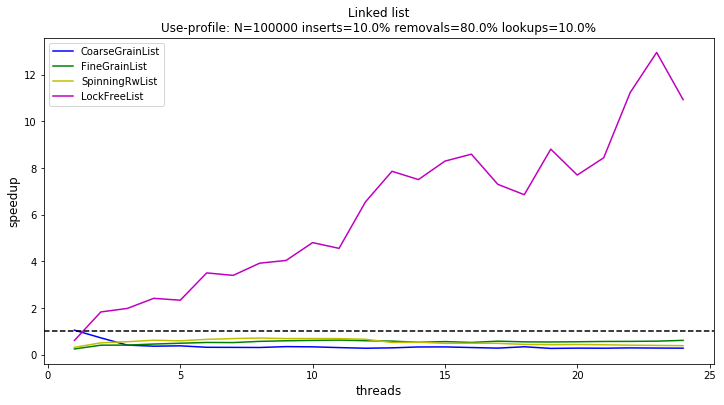
\includegraphics[width=1.0\linewidth]{figs/lateday/combined/lateday_combined_list_insert_10_lookup_10_removal_80}
\caption{Fig.}
\label{fig:fig1}
\end{figure}

\begin{figure}[h]
\centering
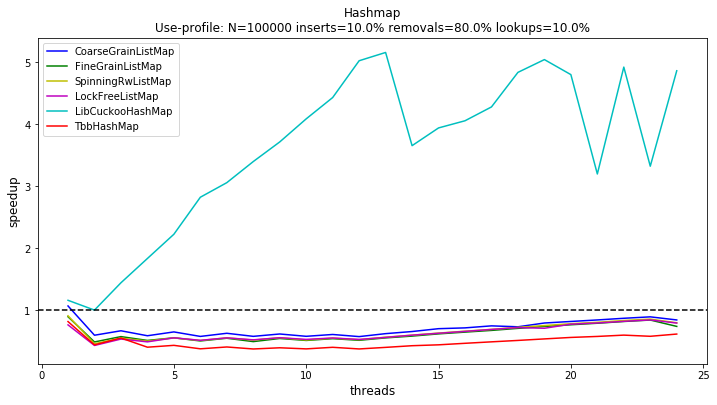
\includegraphics[width=0.5\linewidth]{figs/lateday/combined/lateday_combined_map_insert_10_lookup_10_removal_80}
\caption{Fig.}
\label{fig:fig2}
\end{figure}

\printbibliography

\end{document}
\grid
